\documentclass[a4paper,11pt]{article}

\usepackage[T1]{fontenc}
\usepackage[polish]{babel}
\usepackage[utf8]{inputenc}
\usepackage{lmodern}
\selectlanguage{polish}
\usepackage[top=2cm, bottom=2cm, left=3cm, right=3cm]{geometry}

\makeatletter
\newcommand{\linia}{\rule{\linewidth}{0.4mm}}
\renewcommand{\maketitle}{\begin{titlepage}
    \vspace*{2cm}
    \begin{center}\LARGE
    Politechnika Warszawska\\
    Wydział Elektryczny\\
    \end{center}
    \vspace{5cm}
    \noindent\linia
    \begin{center}
      \LARGE \textsc{\@title}
         \end{center}
     \linia
    \vspace{0.5cm}
    \begin{flushright}
    \begin{minipage}{5cm}
    \textit{Autorzy:}\\
    \normalsize \textsc{\@author} \par
    \end{minipage}
    \vspace{5cm}
     \end{flushright}
    \vspace*{\stretch{6}}
    \begin{center}
    \@date
    \end{center}
  \end{titlepage}%
}
\makeatother
\author{Grzegorz Kopyt\\
Daniel Sporysz}
\title{Sprawozdanie\\
,,WireWorld''}

\usepackage{graphicx}
\begin{document}

\maketitle


\tableofcontents
\vspace{1cm}
\noindent\linia



\section{Opis działania}
XXXXXXXXXXXXXXXXXXXXX

\noindent\linia
\section{Możliwości programu}


\subsection{Edycja planszy}
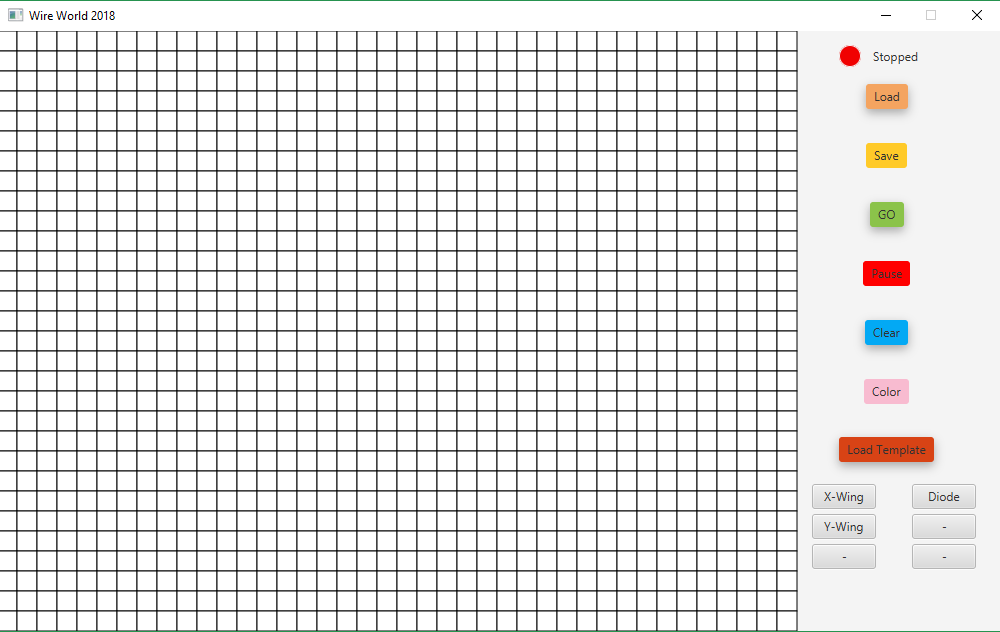
\includegraphics[width=\textwidth]{mainScreen}
\begin{itemize}
\item Zmiana koloru pól poprzez "przeciągnięcie'' - zmieniają się w kolejności pusty->przewodnik->ogon->głowa.
\item Zmiana koloru pól poprzez ''kliknięcie'' lewym przyciskiem myszy - zmieniają się w kolejności pusty->przewodnik->ogon->głowa.
\item Zmiana koloru pól poprzez ''kliknięcie'' prawym przyciskiem myszy - nadanie koloru pusty.
\item Wstawianie gotowych wzorów na plansze poprzez naciśnięcie jednego z przycisków w prawym dolnym rogu i przesuwając kursorem na planszy umieszczenie go w wybranym miejscu i zatwierdzenie lewym przyciskiem myszy lub porzucenie prawym (możliwość obrotu elementów poprzez ''scroll").

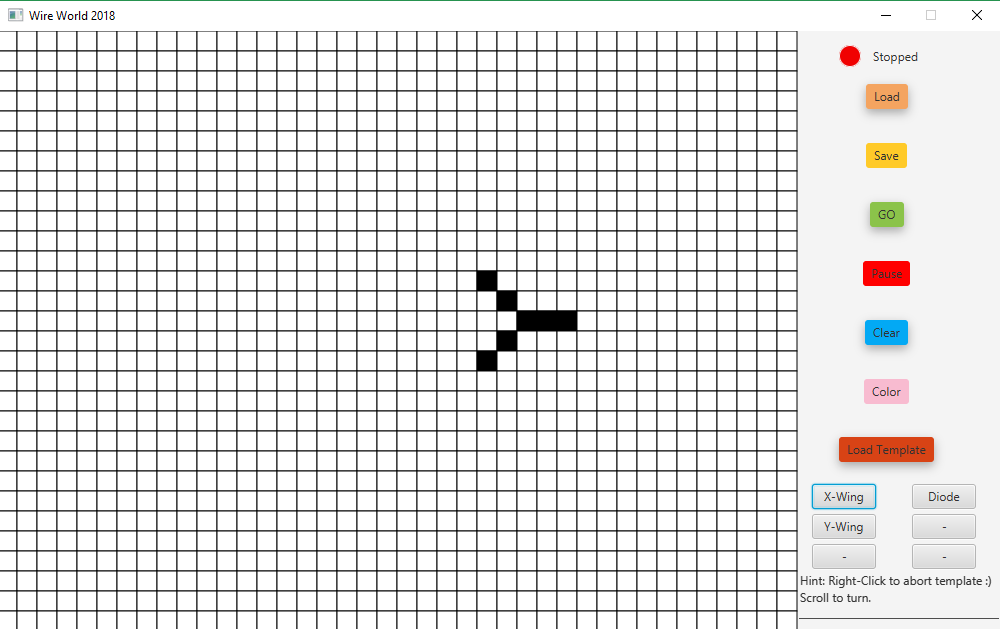
\includegraphics[width=\textwidth]{insertTemplate}
 
\end{itemize}
\subsection{ Zmiana domyślnych kolorów planszy}
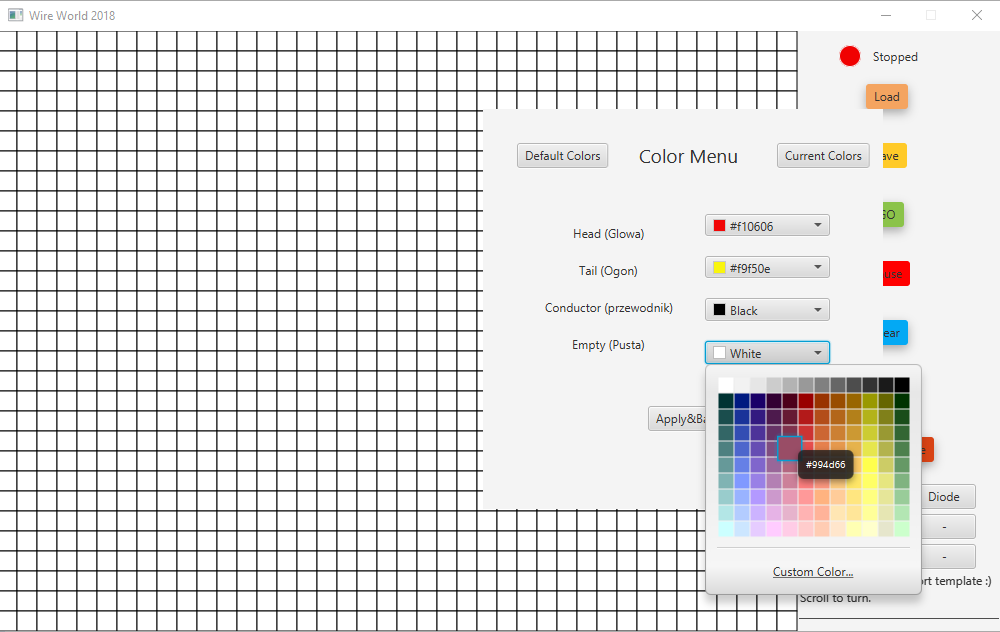
\includegraphics[width=\textwidth]{colorMenu}
\begin{itemize}
\item W wygodnym meny koloru można wybrać własne kompozycje kolorów.
\end{itemize}
\subsection{Dodawanie własnych wzorów}
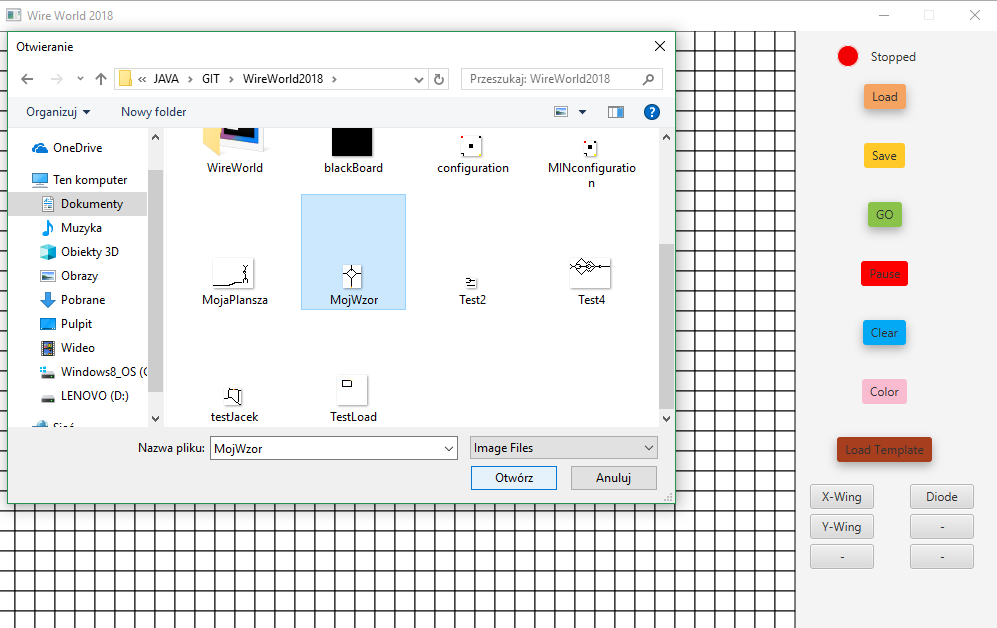
\includegraphics[width=\textwidth]{addWzor1}

\begin{itemize}
\item Możliwość dodania trzech wzorów poprzez przycisk ''LoadTemplate''
\item Nazwa pliku ze wzorem pojawi się na jednym z przycisków w prawym dolnym rogu.

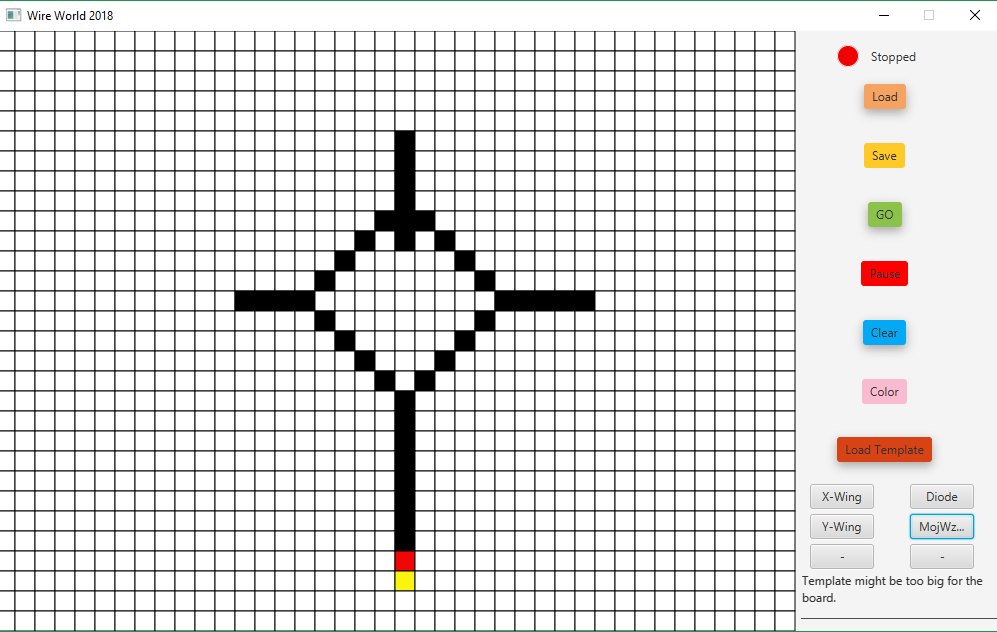
\includegraphics[width=\textwidth]{addWzor2}
\item Plik musi być w formacie graficznym (.png, .jpeg), pokolorowany kolorami biały(pusty), czarny(przewodnik), żółty(ogon), czerwony(głowa)
\end{itemize}

\subsection{Zapis planszy do pliku}
\begin{itemize}
\item Przycisk ''Save'' prowadzi do menu zapisu, gdzie mamy możliwość wyboru nazwy i lokalizacji pliku

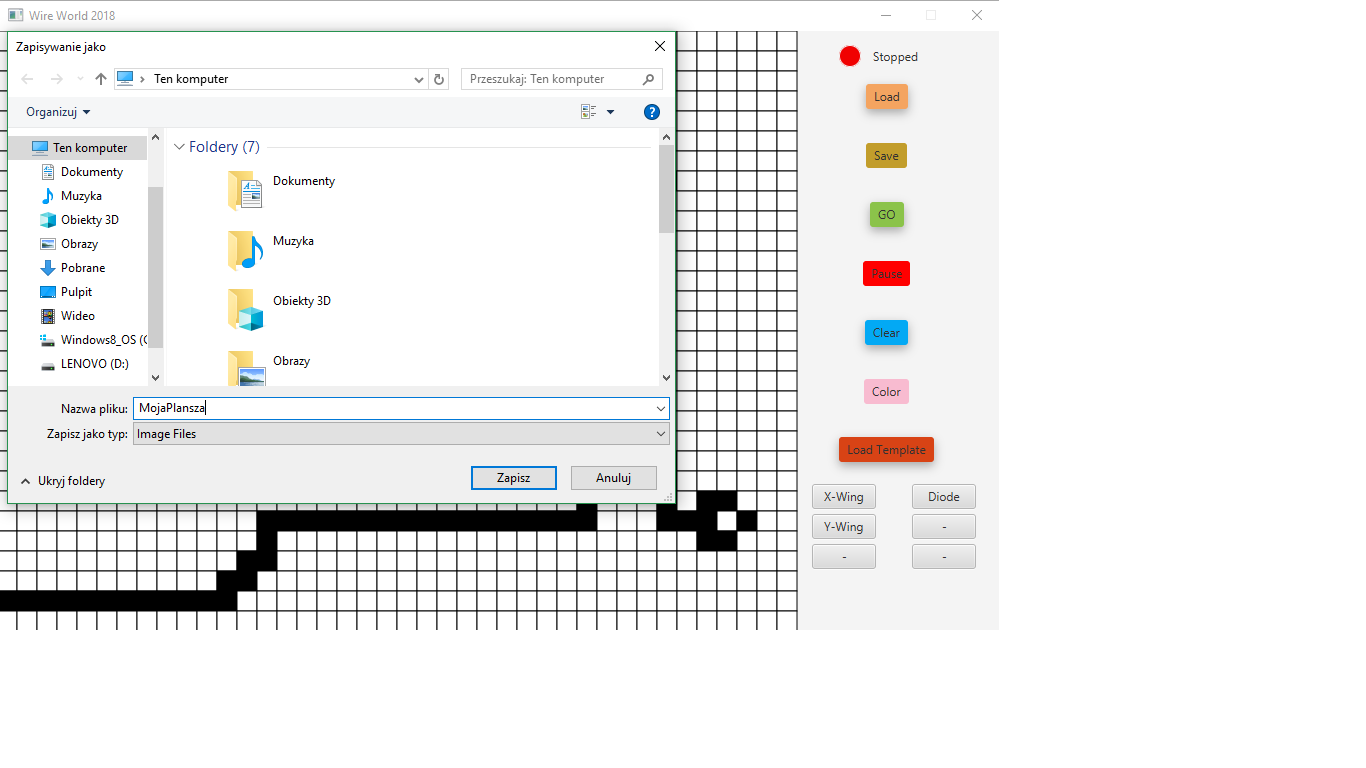
\includegraphics[width=\textwidth]{zapis}
\end{itemize}

\subsection{Wczytanie planszy z pliku}
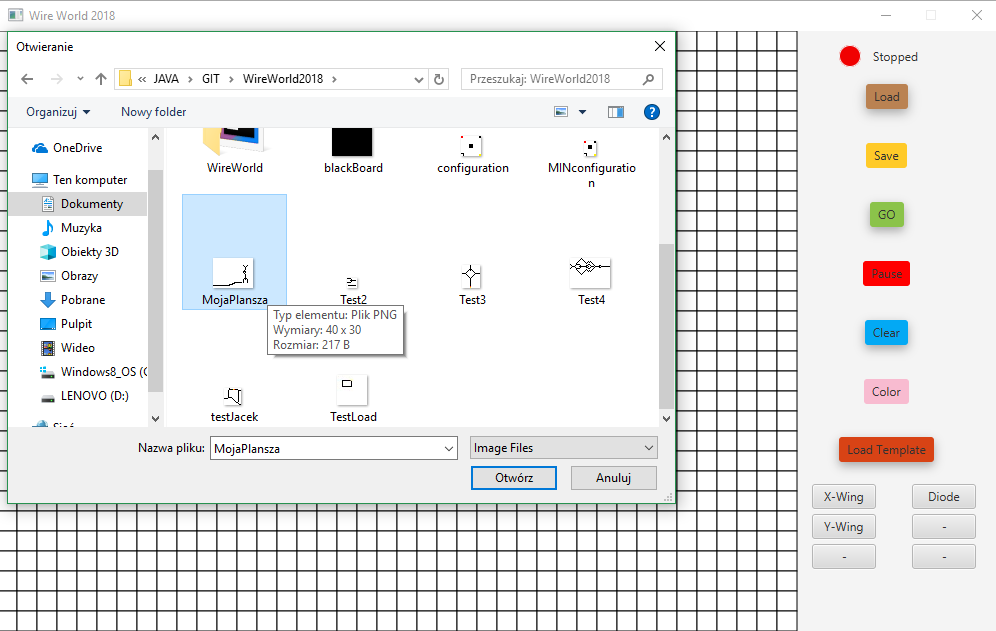
\includegraphics[width=\textwidth]{load}
\begin{itemize}
\item Przycisk 'Load'' prowadzi do menu wyboru plików, gdzie mamy możliwość odnalezienia nazwy i lokalizacji pliku
\item Plik zostaje wczytany i  od razu nałożony na plansze


\end{itemize}
\subsection{Animacja}
\begin{itemize}
\item 
\end{itemize}

\noindent\linia
\section{Opis implementacji}

\subsection{Implementacja modułu ,,Board''}

\begin{enumerate}
\item Wprowadzono klasę Cell rozszerzającą Rectangle, aby móc wyodrębnić w niej metodę zmieniającą kolor, a także pola współrzędnych na planszy danej komórki oraz pole "poprzedniego koloru". Porządkuje to kod i ułatwia korzystanie z klasy Rectangle do naszych celów.
\item Metoda makeBoard otrzymuje dodatkowo jako argumenty wymiary obiektu Pane, na którym będzie tworzona plansza, ponieważ metody inicjujące GUI potrzebowały tej informacji
\item Dodano szereg funkcji pozwalających na kontrolę planszy:
	\begin{itemize}
	\item repaintBoard - nadaje planszy obecne kolory i ustawia "poprzednie kolory" komórek na obecne
	\item setBoardColor - nadaje całej planszy jeden kolor
	\item repaintBoardOnPrevious - maluje komórki planszy na jej poprzednie kolory
	\item setColorMode - ustawia tryb planszy na zwykłe kolorowanie planszy poprzez "kliknięcia" i "przeciągnięcia"
	\item setCurrentBoardMode - nadaje wartość obecnego trybu planszy
	\item setInsensitiveMode - ustawia tryb planszy, w którym jest ona nieczuła na edycje
	\item setTemplateInsertionMode - ustawia tryb planszy na wprowadzanie wzorów
	\end{itemize}

\item W klasie Template zdefiniowano metody wstawiania wzoru na plansze, we wszystkie cztery możliwe kierunki

\end{enumerate}


\subsection{Zmiany w implementacji modułu ,,GUI''}

\begin{enumerate}
\item Do menu wyboru kolorów dodano przycisk powrotu do domyślnych kolorów, a także przycisk ustawienia obecnych kolorów na przyciskach wyboru koloru, co ułatwia zarządzanie kolorami planszy.
\item Do kontrolerów dodano pole Colors , aby przekazywać informacje o obecnych kolorach planszy
\item MainScreenController otrzymał pole BoardMaker, aby przekazywać mu sterowanie naszą planszą
\item MainScreenControlle otrzymał szereg metod kontrolujących elementy tej sceny:
	\begin{itemize}
	\item disableNonTemplateButtons - blokuje dostęp do przycisków nie służących do wstawiania wzorów
	\item disableTemplateButtons - blokuje dostęp do przycisków służących do wstawiania wzorów
	\item isAnimationRunningSignal - pozwala na włączenie lub wyłączenie obiektu pokazującego czy animacja obecnie działa
	\item manageTemplateInsertion - porządkuje działania w metodach pod przyciskami do wstawiania wzorów
	\end{itemize}
\end{enumerate}
\section{Opcje rozbudowy programu}
\begin{enumerate}

\item xxxxxxx

\item xxxxxxx

\end{enumerate}
\end{document}



